% all-in-one cheatsheet layout (Michael Franzen, 2013)
\documentclass[a4paper]{article}

% geometry settings
\usepackage[top=2cm, bottom=2.5cm, left=2cm, right=2cm]{geometry}

% font settings
%\usepackage[light,math]{kurier}
\usepackage[T1]{fontenc}
\usepackage[utf8]{inputenc}
\usepackage{marvosym}
\usepackage{amssymb}
\usepackage{amsfonts}
\usepackage{amsmath}
\usepackage{amsthm}

% colors
\usepackage{xcolor}
\definecolor{lightgray}{gray}{0.8}

% formatting
\usepackage{paralist}
\usepackage{multicol}
\usepackage{tabularx}
\usepackage{Tabbing}
\usepackage{booktabs}
\usepackage{fancyhdr}
\usepackage{url}
\usepackage[framemethod=tikz]{mdframed}
\pagestyle{fancy}

% math
\usepackage{array}
\usepackage{eqnarray}
\usepackage{mathtools}

% figures
\usepackage{wrapfig}
\usepackage{subfig}

% figure modules
\usepackage{graphicx}
\usepackage{tikz}
\usetikzlibrary{positioning,calc, shapes}
\usepackage{algorithm2e}
\usepackage{verbatim}	

% TOC & Glossary
\usepackage{sectsty}
\usepackage[nottoc,notlof,notlot]{tocbibind}
\usepackage[titles,subfigure]{tocloft}

% commands
\usepackage{xargs}
\usepackage{ifthen}

% head line
\fancyhf{}
\chead{Graph Theory - Sheet 3 - \today\\J. Batzill (1698622), M. Franzen (1696933), J. Labeit (1656460)}
\renewcommand{\headrulewidth}{0.4pt} %obere Trennlinie

\newcommand{\sheetnumber}{1}

% (problem number)
\surroundwithmdframed[
    hidealllines=true,
    backgroundcolor=gray!10,
    skipbelow=\baselineskip,
    skipabove=\baselineskip
]{mylemma}

\surroundwithmdframed[
	linecolor=white,
	skipbelow=\baselineskip,
	skipabove=\baselineskip
]{mytheorem}

\tikzstyle{nod}= [circle, draw,inner sep=0pt, minimum size=0.5cm] 

\begin{document}
	
	\newtheorem{mytheorem}{Theorem}[section]
	\newtheorem{mylemma}{Lemma}[mytheorem]	

	\newenvironmentx*{solution}[1]{\section*{Problem #1}\addtocounter{section}{1}\setcounter{mylemma}{0}\setcounter{mytheorem}{0}}{}
	\newenvironmentx*{theorem}[1]{\begin{mytheorem}#1\\\begin{proof}}{\end{proof}\end{mytheorem}}
	\newenvironmentx*{lemma}[1]{\begin{mylemma}#1\\\begin{proof}}{\end{proof}\end{mylemma}}


	\begin{solution}{9}
		\begin{theorem}{A hypercube $Q_n$ is Hamiltonian. It has a girth of $4$ for $n \geq 2$ and $\infty$ otherwise. It's diameter is $n$, it's order $2^n$ and it has a size of $2^{n-1} \cdot n$.}
			Let $S$ be a set of cardinality $|S| = n$. We construct $Q_n = (V_Q, E_Q)$ by creating a vertex for each subset of $S$ and moreover add edges between those subsets which differ by only one element. In the following, we may use binary representations of the vertices of $Q_n$ since $V_Q = \mathcal{P}(S) \cong (\mathbb{Z}/2\mathbb{Z})^n$ (we can denote a $1$ for including an element and a $0$ for excluding an element in a subset).\\

			\textbf{Order:} Since $V_Q = \mathcal{P}(S)$ and $|\mathcal{P}(S)| = 2^n$, \emph{the order of $Q_n$ is $2^n$.}\\

			\textbf{Size:} Each of the $2^n$ vertices is adjacent to $n$ other vertices since we can insert / remove each of the $n$ elements of $S$. For undirected edges, we have $\frac{2^n \cdot n}{2} = 2^{n-1} \cdot n$ edges. \emph{Thus, the size of $Q_n$ is $2^{n-1} \cdot n$.}\\

			\textbf{Girth:} We differentiate between two cases.
				\begin{itemize}
					\item \textbf{Case 1: } $n=1$. Our graph contains exactly one edge and is therefore acyclic. \emph{Hence, the girth is $\infty$ for $n=1$.}

					\item \textbf{Case 2: } $n\geq2$ Our graph contains the cycle ($\emptyset$, $\{a\}$, $\{a,b\}$, $\{b\}$, $\emptyset$) $(a,b \in S)$ which has length $4$.

						A shorter cycle ($A$, $B$, $C$, $A$) $(A, B, C \in V_Q)$ does not exist due to the property that two adjacent vertices differ by exactly one element. For such a cycle, $B$ and $A$ differed by one element, and hence $A$ and $C$ differed by two or are equal. However, a difference of zero or two elements between two consecutive elements renders any walk invalid. The edge $\{C, A\}$ could not be contained in $Q_n$.
 
						\emph{From these considerations, for $n \geq 2$, the girth is $4$.}
				\end{itemize}

			\textbf{Diameter:}
				For any set $A \in V_Q$, we are able to get to any other element $B \in V_Q$ by inserting or removing a maximum of $n$ elements. Thus, a path of length $n$ is sufficient to walk from any $A$ to any $B$. Furthermore, there exist $A$ and $B$ such that a path of length $n$ is the shortest path between them. E.g. $A = \emptyset \in V_Q$, $B = S \in V_Q$. \emph{Thus, the diameter of $Q_n$ is $n$.}\\

			\textbf{Hamiltonian:} A Hamiltonian cycle is equivalent to an enumeration of $(\mathbb{Z}/2\mathbb{Z})^n$ in which consecutive elements differ by exactly one element. We provide such an enumeration: the \emph{Gray Code\footnote{For $n=2$: $00$,$01$,$11$,$10$,$00$. Generally, the $k$'th vertex in the Hamiltonian cycle is $k \otimes \lfloor \frac{k}{2} \rfloor$ whereby $\cdot \otimes \cdot$ denotes the exclusive or.}}. \emph{Thus, there exists a Hamiltonian cycle and $Q_n$ is Hamiltonian.}
		\end{theorem}
		\begin{figure}[h!]
			\begin{center}
				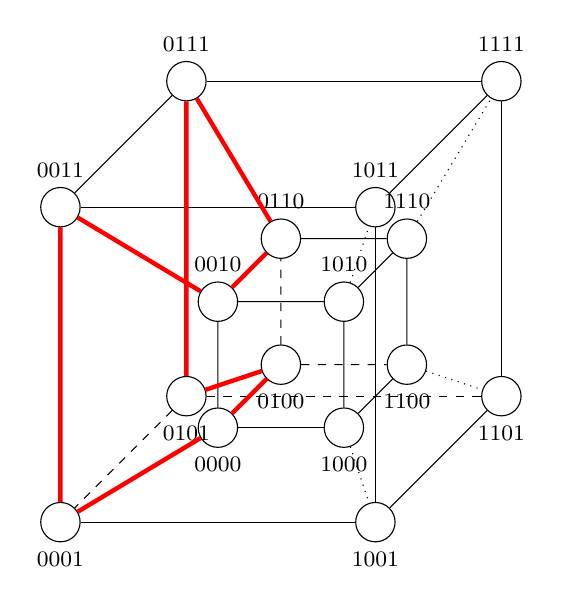
\begin{tikzpicture}[scale=0.8]
					\pgfsetxvec{\pgfpoint{1.cm}{0.0cm}} 
					\pgfsetyvec{\pgfpoint{0.0cm}{1.0cm}} 
					\node[nod] at (0,0) [label=below:\footnotesize$0001$] (0001) {}; 
					\node[nod] at (5,0) [label=below:\footnotesize$1001$] (1001) {}; 
					\node[nod] at (0,5) [label=above:\footnotesize$0011$] (0011) {}; 
					\node[nod] at (5,5) [label=above:\footnotesize$1011$] (1011) {}; 
					\node[nod] at (2,2) [label=below:\footnotesize$0101$] (0101) {}; 
					\node[nod] at (7,2) [label=below:\footnotesize$1101$] (1101) {}; 
					\node[nod] at (2,7) [label=above:\footnotesize$0111$] (0111) {}; 
					\node[nod] at (7,7) [label=above:\footnotesize$1111$] (1111) {}; 
					\node[nod] at (2.5,1.5) [label=below:\footnotesize$0000$] (0000) {}; 
					\node[nod] at (4.5,1.5) [label=below:\footnotesize$1000$] (1000) {}; 
					\node[nod] at (2.5,3.5) [label=above:\footnotesize$0010$] (0010) {}; 
					\node[nod] at (4.5,3.5) [label=above:\footnotesize$1010$] (1010) {}; 
					\node[nod] at (3.5,2.5) [label=below:\footnotesize$0100$] (0100) {}; 
					\node[nod] at (5.5,2.5) [label=below:\footnotesize$1100$] (1100) {}; 
					\node[nod] at (3.5,4.5) [label=above:\footnotesize$0110$] (0110) {}; 
					\node[nod] at (5.5,4.5) [label=above:\footnotesize$1110$] (1110) {}; 
					\path (0011) edge (1011) edge (0111) edge (0001) (1001)	edge (0001) edge (1101) edge (1011) (1111)	edge (1101) edge (1011) edge (0111) (0010) edge (1010) edge (0110) edge (0000) (1000)	edge (0000) edge (1100) edge (1010) (1110)	edge (1100) edge (1010) edge (0110); 
					\path[dashed] (0101) edge (1101)	edge (0001) edge (0111) (0100) edge (1100)	edge (0000) edge (0110); 
					\path[dotted] (0000) edge (0001) (0010) edge (0011) (0100) edge (0101) (0110) edge (0111) (1000) edge (1001) (1010) edge(1011) (1100) edge (1101) (1110) edge (1111); 
					\draw[ultra thick, red] (0000) -> (0001) -> (0011) -> (0010) -> (0110) -> (0111) -> (0101) -> (0100) -> (0000);
				\end{tikzpicture} 
			\end{center} 
			\caption{The hypercube $Q_4$ and the Hamiltonian cycle of $Q_3$ as a subgraph of $Q_4$.}
		\end{figure}

		\newpage		

		\begin{theorem}{A complete bipartite graph $K_{m, n}$ is Hamiltonian iff $m = n$. It's girth is $4$ for $m, n \neq 1$ and and $\infty$ otherwise. It's diameter is $1$ for $m = n = 1$ and $2$ otherwise. The graph's order is $m + n$ and it's size is $m \cdot n$.}
			Let $V = \{v_1, ..., v_m\}$ and $W = \{w_1, ..., w_n\}$ denote the two partitions of $K_{m, n} = (V_K, E_K)$.\\

			\textbf{Order:} The first partition has $m$ elements, the second $n$ elements. \emph{Thus, $K_{m,n}$ has an order of $m + n$.}\\

			\textbf{Size:} Each of the $m$ elements of the first partition are connected to each of the $n$ elements in the second partition. \emph{Thus, $K_{m,n}$ has a size of $m \cdot n$}.\\

			\textbf{Girth:} If either $m=1$ or $n=1$, then all vertices of one partition are indicent to and only to the single vertex of the other partition. Hence, there is no cycle in $K_{1, n}$ or $K_{m, 1}$ and \emph{the girth of $K_{m,n}$ is $\infty$ if $n = 1$ or $m=1$}.\\

				If $m, n \neq 1$, each cycle must have even length since any two consectuive vertices in a path of $K_{n,m}$ are in different partitions. Thus, we require an even amount of edge-crossings to enclose a walk. Any cycle has a length of at least $3$, thus the girth of $K_{m,n}$ has to exceed or be equal to $4$.

				Furthermore, we find such a cycle of length $4$ easily since both partitions $V, W$ have at least $2$ vertices: $(v_1, w_1, v_2, w_2, v_1)$. \emph{From these considerations, the girth of $K_{m,n}$ must be equal to $4$.}\\

			\textbf{Diameter:} For $m = n = 1$, there are exactly two vertices in different partitions. They have a distance of $1$ and thus, \emph{the diameter of $K_{1,1}$ is $1$}.\\

				Since two consectuive vertices in a path of $K_{n,m}$ are in different partitions $V, W$ the distance between two vertices in the same partition has to be at least $2$. Moreover, we find a path of distance $2$ between $v_1 \in V$ to $v_2 \in V$: $(v_1, w, v_2)$ for any $w \in W$. Thus, the diameter does not deceed $2$.

				For any two vertices in different partitions $V, W$, they are directly connected by a path of length $1$.

				 \emph{Hence, the diameter of $K_{m,n}$ is $2$ if not $m = n = 1$}.\\

			\textbf{Hamiltonian:} For $m = n$, we find always find a Hamiltonian cycle: $(v_1, w_1, v_2, w_2, ..., v_n, w_n, v_1)$.

				However, for $m \neq n$, there can not exist a Hamiltonian cycle.

				We assume such a Hamiltonian cycle $c = (u_1, u_2, ..., u_{n+m}, u_1)$ existed for $m \neq n$. 
				\begin{itemize}
					\item \textbf{Case 1:} $m + n$ odd. Then, $u_{n+m}$ and $u_1$ were in the same partition which rendered the edge $\{u_{n+m}, u_1\}$ invalid. \emph{Hence, $K_{m,n}$ is not Hamiltonian for an odd $n + m$.}
					\item \textbf{Case 2:} $m + n$ is even. Then, there was an $n_0 < n+m$ such that $(u_1, ..., u_{n_0})$ is the shortest sub walk that covers one partition but not both. Again, we inspect two cases.
						\begin{itemize}
							\item $\mathbf{n_0 = m + n - 1}$. Then, both partitions have the same number of vertices which is contradictory to our precondition that $m \neq n$.
							\item $\mathbf{n_0 < m + n - 1}$. Then, we are trapped in one partition for we are not able to cover two vertices of the same partition consecutively.
						\end{itemize}
					\emph{Hence, $K_{m, n}$ ($m \neq n$) is not Hamiltonian for an even $m + n$.}
				\end{itemize}

				All in all, $K_{m,n}$ is Hamiltonian if and only if $m = n$.
		\end{theorem}
			
		\newpage
		\begin{theorem}{The Petersen graph is not Hamiltonian, it has a girth of $5$, a diameter of $2$, an order of $10$ and a size of $15$.}
			Let $G = (V, E)$ be the Petersen graph. Then, $V = \binom{\{1, ..., 5\}}{2}$ and $E = \{\{A, B\}\ |\ A \cap B = \emptyset\}$. To avoid loss of generality, we consider that $\{a_1, ..., a_5\} = \{1, ..., 5\}$.
			
			\textbf{Order:} The set $\{1, ..., 5\}$ has $10$ different subsets with $2$ elements each and thus, the number of the graph's vertices and thereby it's order is $10$.\\
			
			\textbf{Size:} Each vertex $\{a_1, a_2\}$ is disjoint to exactly three other $2$-element sets: $\{a_3, a_4\}, \{a_4, a_5\}, \{a_3, a_5\}$. Thus, the graph has $\frac{10 \cdot 3}{2} = 15$ edges and it's size is $15$.\\

			\textbf{Girth:} We consider $C = (\{a_1, a_2\}, \{a_3, a_4\}, ...)$ to be a cycle. $\{a_3, a_4\}$ is disjoint to $\{a_1, a_2\}, \{a_1, a_5\}, \{a_2, a_5\}$. Hence, we inspect the following cases for the continuation of $C$:
			\begin{itemize}
				\item $\mathbf{C = (\{a_1, a_2\}, \{a_3, a_4\}, \{a_1, a_5\}, ...)}$. Then, $C$ is not of length $3$ since $\{a_1, a_5\}$ and $\{a_1, a_2\}$ are not disjoint. Again, we define one case for each subset disjoint to $\{a_1, a_5\}$ (except the vertex' predecessor).
					\begin{itemize}
						\item $\mathbf{C = (\{a_1, a_2\}, \{a_3, a_4\}, \{a_1, a_5\}, \{a_2, a_3\}, ...)}$. Then, $C$ is not of length $4$ since $\{a_2, a_3\}$ and $\{a_1, a_2\}$ are not disjoint.
						\item $\mathbf{C = (\{a_1, a_2\}, \{a_3, a_4\}, \{a_1, a_5\}, \{a_2, a_4\}, ...)}$. Then, $C$ is not of length $4$ since $\{a_2, a_4\}$ and $\{a_1, a_2\}$ are not disjoint.
					\end{itemize}
				\item $\mathbf{C = (\{a_1, a_2\}, \{a_3, a_4\}, \{a_2, a_5\}, ...)}$. Then, $C$ is also not of length $3$ since $\{a_2, a_5\}$ and $\{a_1, a_2\}$ are not disjoint.
					\begin{itemize}
						\item $\mathbf{C = (\{a_1, a_2\}, \{a_3, a_4\}, \{a_2, a_5\}, \{a_1, a_3\}, ...)}$. Then, $C$ is not of length $4$ since $\{a_1, a_3\}$ and $\{a_1, a_2\}$ are not disjoint.
						\item $\mathbf{C = (\{a_1, a_2\}, \{a_3, a_4\}, \{a_2, a_5\}, \{a_1, a_4\}, ...)}$. Then, $C$ is not of length $4$ since $\{a_1, a_4\}$ and $\{a_1, a_2\}$ are not disjoint.
					\end{itemize}
			\end{itemize}
			All in all, the length of the shortest cycle exceeds $4$.

			Since we find a cycle of length $5$, $(\{a_1, a_2\}, \{a_3, a_4\}, \{a_1, a_5\}, \{a_2, a_4\}, \{a_3, a_5\}, \{a_1, a_2\})$, \emph{the girth is $5$}.\\

			\textbf{Diameter:} The distance between two disjoint sets $A, B \in V$ is $1$, since an edge between disjoint vertices exists by definition.
				
				For non-disjoint vertices $A, B \in V$, the sets share exactly one element ($A \cap B \in \{1, ..., 5\}$). Thus, $|A \cup B| = 3$ and there exists a two-element subset $C = \{1, ..., 5\} \setminus (A \cup B)$ which is disjoint to both $A$ and $B$. Finally, $A$ and $B$ can be joined by a path $(A, C, B)$ and the distance is $2$.

				\emph{All in all, the shortest path between any two vertices does not exceed $2$. Thus, the distance of the Petersen graph is $2$.}\\

			\textbf{Hamiltonian:}
			Let's assume the Petersen graph is Hamiltonian, then there would be a cycle containing all 10 nodes. 
			Now we can draw the graph. We start off by drawing the Hamilton cycle. 
			\begin{center}
			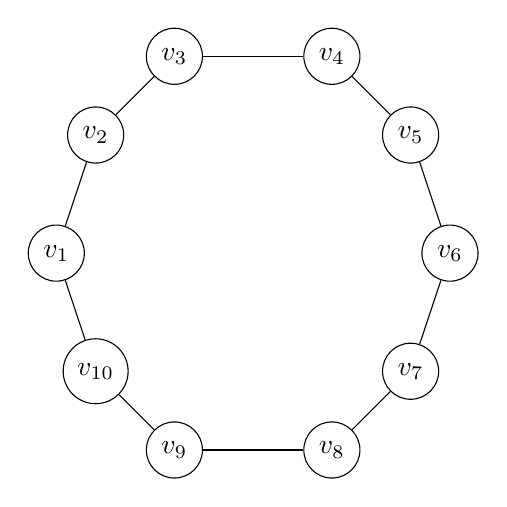
\begin{tikzpicture}
				\node[circle, draw] (v1) at (-2.5, 0) {$v_1$};
				\node[circle, draw] (v2) at (-2, 1.5) {$v_2$};
				\node[circle, draw] (v3) at (-1, 2.5) {$v_3$};
				\node[circle, draw] (v4) at (1, 2.5) {$v_4$};
				\node[circle, draw] (v5) at (2, 1.5) {$v_5$};
				\node[circle, draw] (v6) at (2.5, 0) {$v_6$};
				\node[circle, draw] (v7) at (2, -1.5) {$v_7$};
				\node[circle, draw] (v8) at (1, -2.5) {$v_8$};
				\node[circle, draw] (v9) at (-1, -2.5) {$v_9$};
				\node[circle, draw] (v10) at (-2, -1.5) {$v_{10}$};
				\draw(v1) -- (v2);
				\draw(v2) -- (v3);
				\draw(v3) -- (v4);
				\draw(v4) -- (v5);
				\draw(v5) -- (v6);
				\draw(v6) -- (v7);
				\draw(v7) -- (v8);
				\draw(v8) -- (v9);
				\draw(v9) -- (v10);
				\draw(v10) -- (v1);
			\end{tikzpicture}
			\end{center}
			Now in order for $v_1$ to have degree 3, the graph must have another edge. 
			We already know that the minimum cycle in the Petersen graph is of length $5$ so $v_1$ can only be connected to $v_5$,$v_6$ or $v_7$. 
			Because of symmetry reasons, we only need to consider the following two cases. 
			\begin{itemize}
				\item \emph{$(v_1,v_5)$ is an edge of Petersen Graph}\\
					Then either $(v_{10},v_4)$, $(v_{10},v_5)$ or $(v_{10},v_6)$ has to be part of the Petersen graph. 
					In all three cases a cycle is created with a size smaller than 5. 
					($v_1,v_5,v_4,v_{10},v_1$ with edge $(v_{10},v_4)$,  $v_1,v_5,v_{10},v_1$ with edge $(v_{10},v_5)$ or $v_1,v_5,v_6,v_{10},v_1$ with edge $(v_{10},v_6)$ )
					In conclusion, the edge $(v_1,v_5)$ cannot be part of the Petersen graph. 
					\begin{center}
					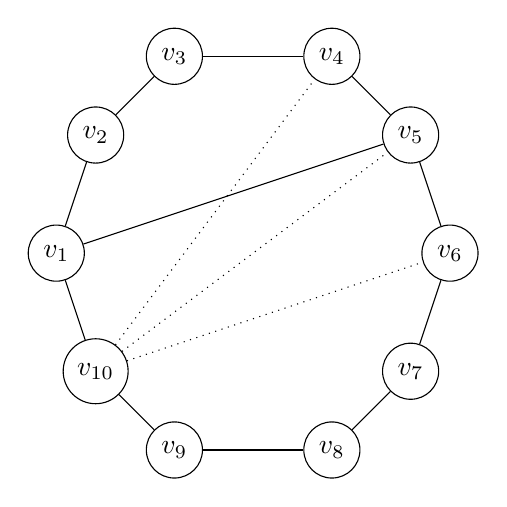
\begin{tikzpicture}
						\node[circle, draw] (v1) at (-2.5, 0) {$v_1$};
						\node[circle, draw] (v2) at (-2, 1.5) {$v_2$};
						\node[circle, draw] (v3) at (-1, 2.5) {$v_3$};
						\node[circle, draw] (v4) at (1, 2.5) {$v_4$};
						\node[circle, draw] (v5) at (2, 1.5) {$v_5$};
						\node[circle, draw] (v6) at (2.5, 0) {$v_6$};
						\node[circle, draw] (v7) at (2, -1.5) {$v_7$};
						\node[circle, draw] (v8) at (1, -2.5) {$v_8$};
						\node[circle, draw] (v9) at (-1, -2.5) {$v_9$};
						\node[circle, draw] (v10) at (-2, -1.5) {$v_{10}$};
						\draw(v1) -- (v2);
						\draw(v2) -- (v3);
						\draw(v3) -- (v4);
						\draw(v4) -- (v5);
						\draw(v5) -- (v6);
						\draw(v6) -- (v7);
						\draw(v7) -- (v8);
						\draw(v8) -- (v9);
						\draw(v9) -- (v10);
						\draw(v10) -- (v1);
						\draw(v1) -- (v5);
						\draw[dotted](v10) -- (v4);
						\draw[dotted](v10) -- (v5);
						\draw[dotted](v10) -- (v6);
					\end{tikzpicture}
					\end{center}
				\item \emph{$(v_1,v_6)$ is an edge of Petersen Graph}\\
					By examining $v_2$, we see that $v_2$ can only be connected to $v_8$. Otherwise, there would be a cycle of size smaller than 5. 
					Then, examining $v_3$, we see that $v_3$ can neither be connected to $v_7$, $v_8$ nor $v_9$ because in every case there would be a cycle of size smaller than 5. 
					In conclusion, the edge $(v_1,v_6)$ cannot be part of the Petersen graph. 
					\begin{center}
					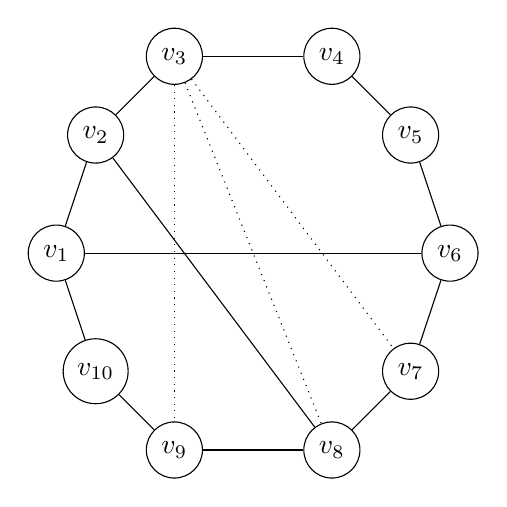
\begin{tikzpicture}
						\node[circle, draw] (v1) at (-2.5, 0) {$v_1$};
						\node[circle, draw] (v2) at (-2, 1.5) {$v_2$};
						\node[circle, draw] (v3) at (-1, 2.5) {$v_3$};
						\node[circle, draw] (v4) at (1, 2.5) {$v_4$};
						\node[circle, draw] (v5) at (2, 1.5) {$v_5$};
						\node[circle, draw] (v6) at (2.5, 0) {$v_6$};
						\node[circle, draw] (v7) at (2, -1.5) {$v_7$};
						\node[circle, draw] (v8) at (1, -2.5) {$v_8$};
						\node[circle, draw] (v9) at (-1, -2.5) {$v_9$};
						\node[circle, draw] (v10) at (-2, -1.5) {$v_{10}$};
						\draw(v1) -- (v2);
						\draw(v2) -- (v3);
						\draw(v3) -- (v4);
						\draw(v4) -- (v5);
						\draw(v5) -- (v6);
						\draw(v6) -- (v7);
						\draw(v7) -- (v8);
						\draw(v8) -- (v9);
						\draw(v9) -- (v10);
						\draw(v10) -- (v1);
						\draw(v1) -- (v6);
						\draw(v2) -- (v8);
						\draw[dotted](v3) -- (v7);
						\draw[dotted](v3) -- (v8);
						\draw[dotted](v3) -- (v9);
					\end{tikzpicture}
					\end{center}
			\end{itemize}
			Because of the symmetry of the cycle, we can conclude that there is no way to construct the Petersen graph from a cycle with 10 vertices.
			\emph{Thus, we know that the Petersen graph cannot be Hammiltonian.}
		\end{theorem}
	\end{solution}
	\newpage
	\begin{solution}{11}
		In the following, I will show how to construct for each $k>1$ a k-regular graph with no 1-factor. 
		The basic idea is that for even $k$, simply $K_{n+1}$ is such a graph. 
		For odd $k$,  I will show a way how to build such a $k-regular$ graph by connecting one vertex to $k$ components with odd number of vertices.  \\ 
		
		For each even integer $k > 1$, the complete graph $K_{k+1}$ is a $k$-regular graph without a $1$-factor. 
		$K_{k+1}$ is by definition $k$-regular and because $K_{k+1}$ has a odd number of components if $k$ is even, it is obviously impossible to find a 1-factor. 
		For each odd $k > 1$, we are able to construct a $k$-regular graph without a $1$-factor in the following way. \\
		
		In order to guarantee that the graph has no $1$-factor, we can use Tutte's theorem. We construct the graph by starting with a single vertex $v \in V$ connected to $k$ subgraphs $S$ which are not inter-connected. 
		\begin{figure}[h]
			\centering
			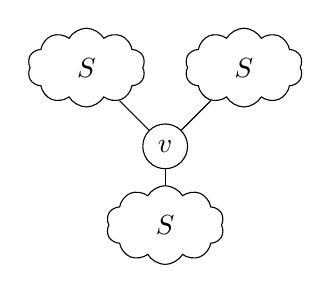
\begin{tikzpicture}
				\node[cloud, cloud puffs=10, cloud puff arc=120, aspect=2, minimum width=1.5cm, minimum height=1cm, draw] (S1)  at (0,-1.0) {$S$};
				\node[cloud, cloud puffs=10, cloud puff arc=120, aspect=2, minimum width=1.5cm, minimum height=1cm, draw] (S2)  at (-1.0,1.0) {$S$};
				\node[cloud, cloud puffs=10, cloud puff arc=120, aspect=2, minimum width=1.5cm, minimum height=1cm, draw] (S3)  at (1.0,1.0) {$S$};

				\node[circle, draw] (v) at (0, 0) {$v$};
				\draw(v) -- (S1);
				\draw(v) -- (S2);
				\draw(v) -- (S3);
			\end{tikzpicture}
			\hfill
			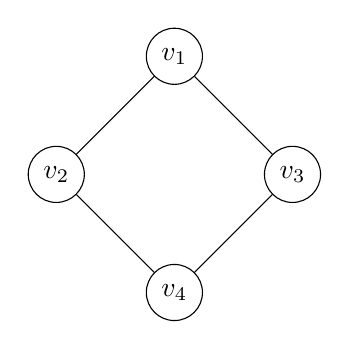
\begin{tikzpicture}
				\node[circle, draw] (v1) at (0, 1.5) {$v_1$};
				\node[circle, draw] (v2) at (-1.5, 0) {$v_2$};
				\node[circle, draw] (v3) at (1.5, 0) {$v_3$};
				\node[circle, draw] (v4) at (0, -1.5) {$v_4$};
				
				\draw(v1) -- (v2);
				\draw(v1) -- (v3);
				\draw(v3) -- (v4);
				\draw(v2) -- (v4);
			\end{tikzpicture}
			\hfill
			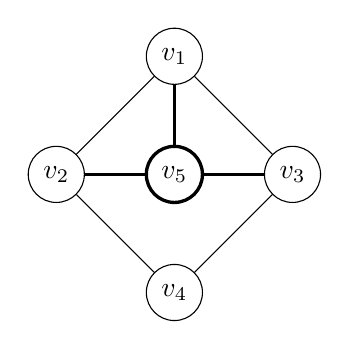
\begin{tikzpicture}
				\node[circle, draw] (v1) at (0, 1.5) {$v_1$};
				\node[circle, draw] (v2) at (-1.5, 0) {$v_2$};
				\node[circle, draw] (v3) at (1.5, 0) {$v_3$};
				\node[circle, draw] (v4) at (0, -1.5) {$v_4$};
				\node[circle, draw,very thick] (v5) at (0, 0) {$v_5$};
				
				\draw(v1) -- (v2);
				\draw(v1) -- (v3);
				\draw(v3) -- (v4);
				\draw(v2) -- (v4);
				\draw[very thick](v5) -- (v1);
				\draw[very thick](v5) -- (v2);
				\draw[very thick](v5) -- (v3);
			\end{tikzpicture}
		\caption{G, S' and S for k=3}
		\end{figure}
		Then, we construct $S=(V,E)$ in such a way that $|V|$ is odd and exactly one vertex $u \in V$ has degree $k-1$ while all other vertices have degree $k$.
 
		If we then connect $u$ to $v$, we obtain a $k$-regular graph. If we removed $v$ we would have $k$ components $S$ with an odd number of vertices. Furthermore, $k > 1$ and thus, by Tutte's theorem, we know that the resulting graph has no $1$-factor.\\
		
		In order to construct $S$ we first need the following lemma.
		\begin{lemma}{For any odd integer $k > 1$ it is possible to construct a $(k-1)$-regular graph $G=(V,E)$ with $k+1$ vertices.}
			We can obtain $G$ from $K_{k+1}$ by removing all edges from $K_{k+1}$ which are contained in a perfect matching of $K_{k+1}$. 

			By removing those edges, the degree of every vertex decreases exactly by one. 
			$K_{k+1}$ is by definition $k$-regular and hence $G$ is $k-1$-regular.

			A perfect matching in $K_{k+1}$ exists, because $k+1$ is even, and the conditions of Tutte's theorem are always satisfied in a complete graph. Moreover, we find such a matching by randomly choosing edges $\{u,v\}$ and removing $u$ and $v$ from $K_{k+1}$. 
		\end{lemma}
		
		\emph{Constructing a connected graph $S=(V,E)$ with $|V|=k+2$ and the degree sequence $( k,k,...,k,(k-1))$. }  
		First we construct a $(k-1)$-regular graph $S' = (V',E')$ with $k+1$ vertices as described in the aforementioned way. Then, we can add one vertex to $S'$ and connect it to all except one vertices in $V'$. Thus, we have a new graph $S$. 
		Because we have added only one vertex $|V| = |V'| +1 = k+2$ and the degree of the newly added vertex is $k$, the degree of all the other vertices except of the last one is increased by one.\\

		Hence, $S$ hat the degree sequence $(k,k,...,k,(k-1))$. 
		By connecting one vertex to $k$ subgraphs isomorph to S, like described above, we have constructed a $k$-regular graph without a perfect matching.
	\end{solution}
	\newpage
	\begin{solution}{12}
		\begin{theorem}{Any graph $G$ with $2n$ vertices and $\delta(G) \geq n$ has a $1$-factor.}
			Let $G=(V,E)$ be a graph with $|V| = 2n$ and $d(v) \geq n \: \forall v \in V$.

			In the following, we will prove for nontrivial $G$ that the number of odd components in a graph $G - S$ deceeds the number of vertices in S. By \emph{Tutte's Matching Theorem}, $G$ then has a $1$-factor.
			\begin{itemize}
				\item [$\mathbf{n = 1}$]

					Then, $G$ is a simple graph with two vertices that are connected by one edge. This is of course a perfect matching of $G$.
			
				\item [$\mathbf{n \geq 2}$]

					Let $S \subseteq V$ be a set of vertices, $G' = (V', E') := G - S$ and $k := |S|$.\\
					As $G'$ is created by removing all vertices of $S$ and their incident edges from $G$, we obtain the following properties: 
					\begin{itemize}
						\item $\forall v \in V: d(v) \geq n - k$
						\item For any component $C$ of $G'$, $|V(C)| \geq n-k+1$
						\item the order of G is $2n-k$
					\end{itemize}
					
					In the following cases, we prove that $\lambda:=\#odd\ components \leq k$.
					\begin{itemize}
						\item[$\mathbf{k=0}$]:

							Because $G$ consists of one even component, $\lambda=0 \leq k$
						\item[$\mathbf{k=1}$]:

							After removing any vertex of $G$, the degree of a vertex in $G'$ is reduced by one or less. Hence, $\forall v \in V: d(v) >= n-1$. This implies that the size of any component in $G'$ is at least $n$. As far as $|V'|=2n-1$ there can only exist one component in $G'$ with order $2n-1$ (which is odd).

							All in all, we have shown that $\lambda=1 \leq k$.
						
						\item[$\mathbf{2\leq k \leq n}$]:

							As the minimum size of a component in $G'$ is $n-k+1$ and $|V'|=2n-k$, we can bound the amount of components by the following term: $\frac{2n-k}{n-k+1}$.

							We now have to prove that 
							$\frac{2n-k}{n-k+1} \leq k \iff 2n-k \leq k*n-k^2+k \iff 0 \leq (k-2)n-k^2+2k =: f(k)$.

							To prove this inequality, we have to determine the minimum value of $f$ in the defined boundaries.
							\begin{itemize}
								\item $f'(k)=n-2k+2 =^! 0 \iff k=\frac{n}{2}+1$
								\item $f''(k)=-2$
							\end{itemize}
							So $f$ has a maximum but no local minimum. To find the minimum value within the given range, we have to check the borders:

							$f(2)=0=f(n)$. Thus, $\min(f)=0 \geq f(k)$ which proves the inequality.

							All in all, we have shown that the number of compomonents deceeds or is equal to $k$. This implies that $\lambda \leq k$.
					\item[$\mathbf{n \leq k \leq 2n}$]:

						Because the number of components can not exceed the number of vertices and $V'=2n-k\leq n \leq k$, there can not  be more than k odd components.

						Hence, $\lambda \leq k$.
				\end{itemize}
				Finally, we have shown that the number of resulting components in $G'$ is bounded by the order of $S$.
				In other words: $\forall  S \subseteq V(G): \#odd\ components\ of\ G-S \leq |S|$.\\

				Thus, we have shown that all conditions for \emph{Tutte's Matching Theorem} are satisfied. Hence, $G$ has a pefect matching aka $1$-factor.
			\end{itemize}
		\end{theorem}
	\end{solution}
	
\end{document}
